\begin{problem}
  Finish the Laplace equation
  \begin{align}\label{laplace}
    -\triangle u &= f(x) \quad \text{on $\Omega$} \notag \\
    u &= 0 \quad \text{on $d\Omega$}
  \end{align}
  solution by finite element
  space using the seven hat functions on hexagons as a basis where $f(x) = -x + 1$.
\end{problem}

\begin{proof}
  We wish to find an approximation to the exact solution $u(x, y)$ in the form
  \[
    u_7(x, y) = \sum_{i=0}^6 a_i \phi_i(x, y)
  \]
  where $\phi_j(x, y)$ are the hat functions with support on the hexagon of definition, i.e.
  we define $\phi_j(x)$ to be 1 on the center nodes of the hexagon and 0 on the boundary.
  Refer to Figure \ref{mesh} for the location of the nodes of these basis functions.
  Note that for the triangles in the mesh the basis functions form a plane whose equation we must define.


  \begin{figure}[!h]
    \begin{center}
      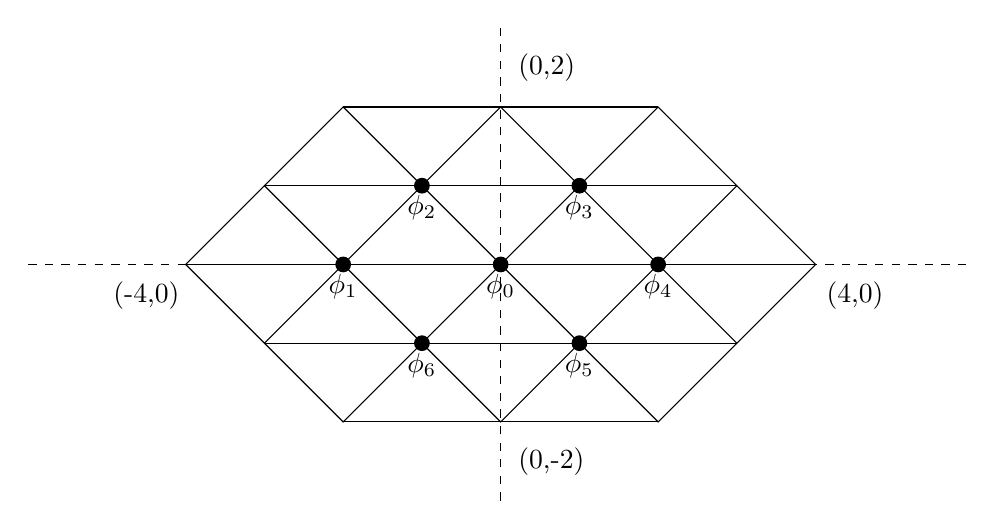
\begin{tikzpicture}
        % Draw mesh grid.
        \draw (-2, 2) -- (0, 2) -- (2, 2);
        \draw (-3, 1) -- (-2, 2) -- (-1, 1) -- (0, 2) -- (1, 1) -- (2, 2) -- (3, 1);
        \draw (-3, 1) -- (-1, 1) -- (1, 1) -- (3, 1);
        \draw (-4, 0) -- (-3, 1) -- (-2, 0) -- (-1, 1) -- (0, 0) -- (1, 1) -- (2, 0) -- (3, 1) -- (4, 0);
        \draw (-4, 0) -- (-2, 0)  -- (0, 0)  -- (2, 0)  -- (4, 0);
        \draw (-4, 0) -- (-3, -1) -- (-2, 0) -- (-1, -1) -- (0, 0) -- (1, -1) -- (2, 0) -- (3, -1) -- (4, 0);
        \draw (-3, -1) -- (-1, -1) -- (1, -1) -- (3, -1);
        \draw (-3, -1) -- (-2, -2) -- (-1, -1) -- (0, -2) -- (1, -1) -- (2, -2) -- (3, -1);
        \draw (-2, -2) -- (0, -2) -- (2, -2);

        % Draw x-y axis
        \draw [dashed] (-6, 0) -- (6, 0);
        \draw [dashed] (0, -3) -- (0, 3);

        % Draw nodes
        \fill (0,0) circle (0.1) node[below]{$\phi_0$};
        \fill (-2,0) circle (0.1) node[below]{$\phi_1$};
        \fill (-1,1) circle (0.1) node[below]{$\phi_2$};
        \fill (1,1) circle (0.1) node[below]{$\phi_3$};
        \fill (2,0) circle (0.1) node[below]{$\phi_4$};
        \fill (1,-1) circle (0.1) node[below]{$\phi_5$};
        \fill (-1,-1) circle (0.1) node[below]{$\phi_6$};

        \fill (-4.5,-0.1) node[below]{(-4,0)};
        \fill (4.5,-0.1) node[below]{(4,0)};
        \fill (0.1, -2.5) node[right]{(0,-2)};
        \fill (0.1, 2.5) node[right]{(0,2)};
      \end{tikzpicture}
    \end{center}
    \caption{Finite element mesh for the 7 hat functions centered at $(0, 0)$.}\label{mesh}
  \end{figure}

  As discussed in class, the weak formulation of the differential equation
  \label{laplace} is as follows
  \[
    \int_\Omega \triangledown u(x, y) \cdot \triangledown\phi_i(x, y) d\Omega = \int_\Omega f(x)\phi_i(x, y)d\Omega \quad \text{for $i=0,\dots,6$}.
  \]
  Discretizing the solution $u(x, y)$ with the approximation $u_7(x, y)$, we
  then require our approximation to satisfy the following system
  \begin{align}\label{laplace_system}
    \sum_{j=0}^6 a_j \int_\Omega \triangledown \phi_j(x, y) \cdot \triangledown \phi_i(x, y) d\Omega = \int_\Omega f(x)\phi_i(x, y)d\Omega \quad \text{for $i=0,\dots,6$}.
  \end{align}
  This system is then given by $Ax = b$ where $A = [a_{ij}]$ is the stiffness matrix
  of the differential equation with $a_{ij} = \int_\Omega \triangledown \phi_j(x, y) \cdot \triangledown \phi_i(x, y) d\Omega$
  and $b = [b_i]$ with $b_i = \int_\Omega f(x)\phi_i(x, y)d\Omega$ for $i=0,\dots,6$. The vector $x$ is the solution vector of the system
  and defines the coefficients in our approximation.


\end{proof}
